\documentclass{article}
\usepackage[T1]{fontenc}
\usepackage{graphicx}
%\usepackage{pgfplots}
%\usepackage[OT4,plmath]
\usepackage{epstopdf}
\usepackage{amsmath,amssymb,amsfonts,amsthm}
\usepackage[utf8]{inputenc}
%\usepackage[english]{babel}
\newcommand\tab[1][1cm]{\hspace*{#1}}
\usepackage{hyperref}
\usepackage{color}
\usepackage{algorithm2e}
\usepackage[margin=1.25in]{geometry}
\usepackage[figurename=Wykres]{caption}
\DeclareMathSizes{12}{30}{16}{12}
%\usepackage[scaled=1.5]{helvet}

\title{Lista 12, Zadanie 1,2}
\author{Wojciech Ganobis 310519}
\date{02/06/20}

\begin{document}
\maketitle

\section{Zadanie}
W zadaniu pierwszym mamy obszar krytyczny określony nierównością $z > 2$. Musimy sprawdzić jaki będzie nasz poziom istotności $\alpha$. Wykres rozkładu normalengo $N(0,1)$ to:
\begin{figure}[h]
	\centering
   
		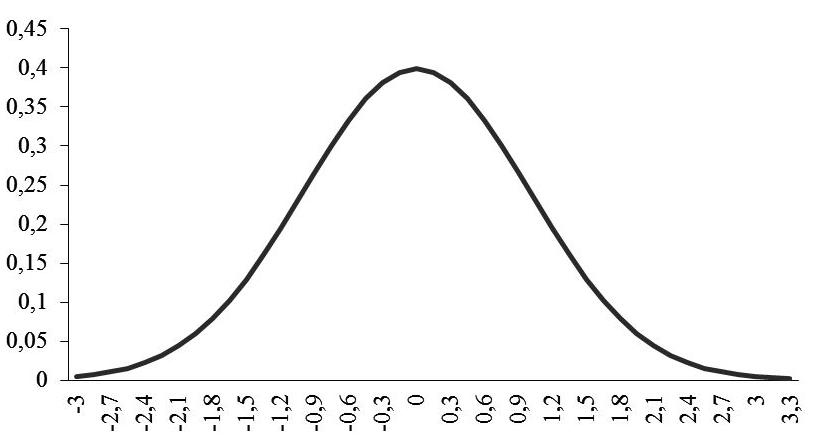
\includegraphics[width=8cm]{plot1}
		\caption{N(0,1)}
\end{figure}
Określmy nasze $Z$ jako $Z \thicksim N(0,1)$.
Teraz podstawmy do wzoru:\\
$$P(Z > 2) = 1 - P(Z \leq 2) = 1 - 0,9772 = 0,0228$$
Czyli nasze $\alpha =  0,0228$, odpoweiedź b.\\\\\\
\section{Zadanie}
Tym razem mamy nierówność $|z| > 1,55$.
Teraz liczymy:
$$P(|Z| > 1,55) = P(Z < -1.55) + P(Z > 1.55) = 0.0606 + 1 - P(Z \leq 1.55) = 1.0606 - 0.9394 = 0.1212$$
Nasze $\alpha$ to 0.1212 czyli odpowieź c.


\end{document}
